\documentclass[12pt]{article}

\usepackage{colortbl}
\usepackage{amsmath}
\usepackage{amssymb}
\usepackage{appendix}
\usepackage{subfigure}
\usepackage{empheq}
\usepackage{framed}
\usepackage[USenglish]{babel}
\usepackage{graphicx}
\usepackage[margin=1.0in]{geometry}
\setcounter{tocdepth}{3}

\usepackage{pdfpages}

\usepackage{eurosym}
\usepackage{mathpazo} 
\usepackage{booktabs}

\def\betabold{{\pmb{$\beta$}}}

%
\begin{document}

\date{August 30 , 2023}

\title{
\centerline{}
\centerline{}
\centerline{}
ETEAPOT PTR Benchmark I: Updated Results:
}
\author{J. D. Talman and R. M. Talman
}

\maketitle

% \tableofcontents

\begin{abstract}
This chapter repeats and updates benchmark lattice investigations first performed 
using the ``all-electric'' code ETEAPOT in 2012 for all-electric proton EDM rings. 
Recently introduced is the extension to ``predominantly electric bending''; this extension
has not influenced this PTR Benchmark I.  The lattice electric bending fields for three PTR 
files have field shape indices $m=0.19447, 0.29447, 0.32349, 0.39447$.  Values of horizontal and vertical 
tunes, and beta functions at the origin (midway between adjacent bends) are tabulated. 
Results are compared to values obtained from a linearized transfer matrix formalism.
\end{abstract}
%

\clearpage

\section{Introduction}
All-electric lattices for a storage ring to measure the electric dipole moment (EDM) of the proton, 
now generalized to support the superposition of weak magnetic bending to enable storage ring 
measurement of nuclear transmutation, are described in a CERN Yellow Report, CERN-2019-001-M, 
``Feasibility Study for a Storage Ring to Search for EDMs of Charged Particles''.  Earlier designs 
were contained in a BNL proposal by the Storage Ring EDM Collaboration, 
\emph{A Proposal to Measure the Proton Electric Dipole Moment with $10^{-29}\,$e-cm Sensitivity}\cite{pEDM}.  
The lattices studied here have been stripped down to their bare essentials in order to simplify benchmark 
comparisons of various simulation codes. All results use ETEAPOT, as described in an (unpublished) 2012 
benchmark report (to the DOE, in connection with their financial support at the time).  They are replicated 
using (updated) ETEAPOT in the present report. 

An electric field with index $m$ power law dependence on radius $r$ for $y$=0, is
%
\begin{equation}
{\bf E}(r,0)
 = 
-E_0\,\frac{r_0^{1+ m }}{r^{1+ m }}\,{\bf\hat r},
\label{eq:WeakFoc.1m}
\end{equation}
%
and the electric potential $V(r)$, adjusted to vanish (on the storage ring 
design orbit) at $r=r_0$, is 
%
\begin{equation}
V(r)
 =
-\frac{E_0r_0}{ m }\,
\bigg(
\frac{r_0^m }{r^m }
 -
1
\bigg).
\label{eq:WeakFoc.2m}
\end{equation}
%
By convection $E_0$ is positive, even though the electric field applies centripetal force
to all nuclear isotopes including the proton.

The ``cleanest'' case theoretically has $m$=1, in which case the field is known
as the Kepler or the Coulomb electric field. Our problem is a
bit more general than this non-reletivistic terminology suggests, since our
treatment is necessarily relativistic. For $m$=1 the
Kepler problem can be solved with the same generality
in the relativistic as in the nonrelativistic case.  However,  the
orbits are no longer exactly elliptical, nor exactly closed
\cite{Munoz}.

The full rings simulated in this chapter are circular and consist of eight octants,
each containing a single almost  identical  half cell.  A single bending element , with toroidally-shaped 
electrodes is shown in perspective in Figure~\ref{fig:SectorPerspective}.  Also shown in the figure, though 
not used in this benchmark I report, are coils for superimposing  magnetic field.  For field index $m$=0 the 
electrodes are concentric cylinders.  For $m$=1 the electrodes would be concentric spheres.  The most 
promising behavior is expected to lie in the range $0.1<m<0.45$.  

A PTR lattice layout is shown in Figure~\ref{fig:PTR-layout-Toroidal8_102p2-mod}.
Optics for one quadrant (with arc length parameter $s$ taken as a Cartesion straight
line coordinate) are shown on the left.  One quadrant of the same lattice is shown 
in perspective view in Figure~\ref{fig:PTR-layout-Toroidal8_102p2-mod}. 

\clearpage

%
\vskip -1cm
\begin{figure}
\centering
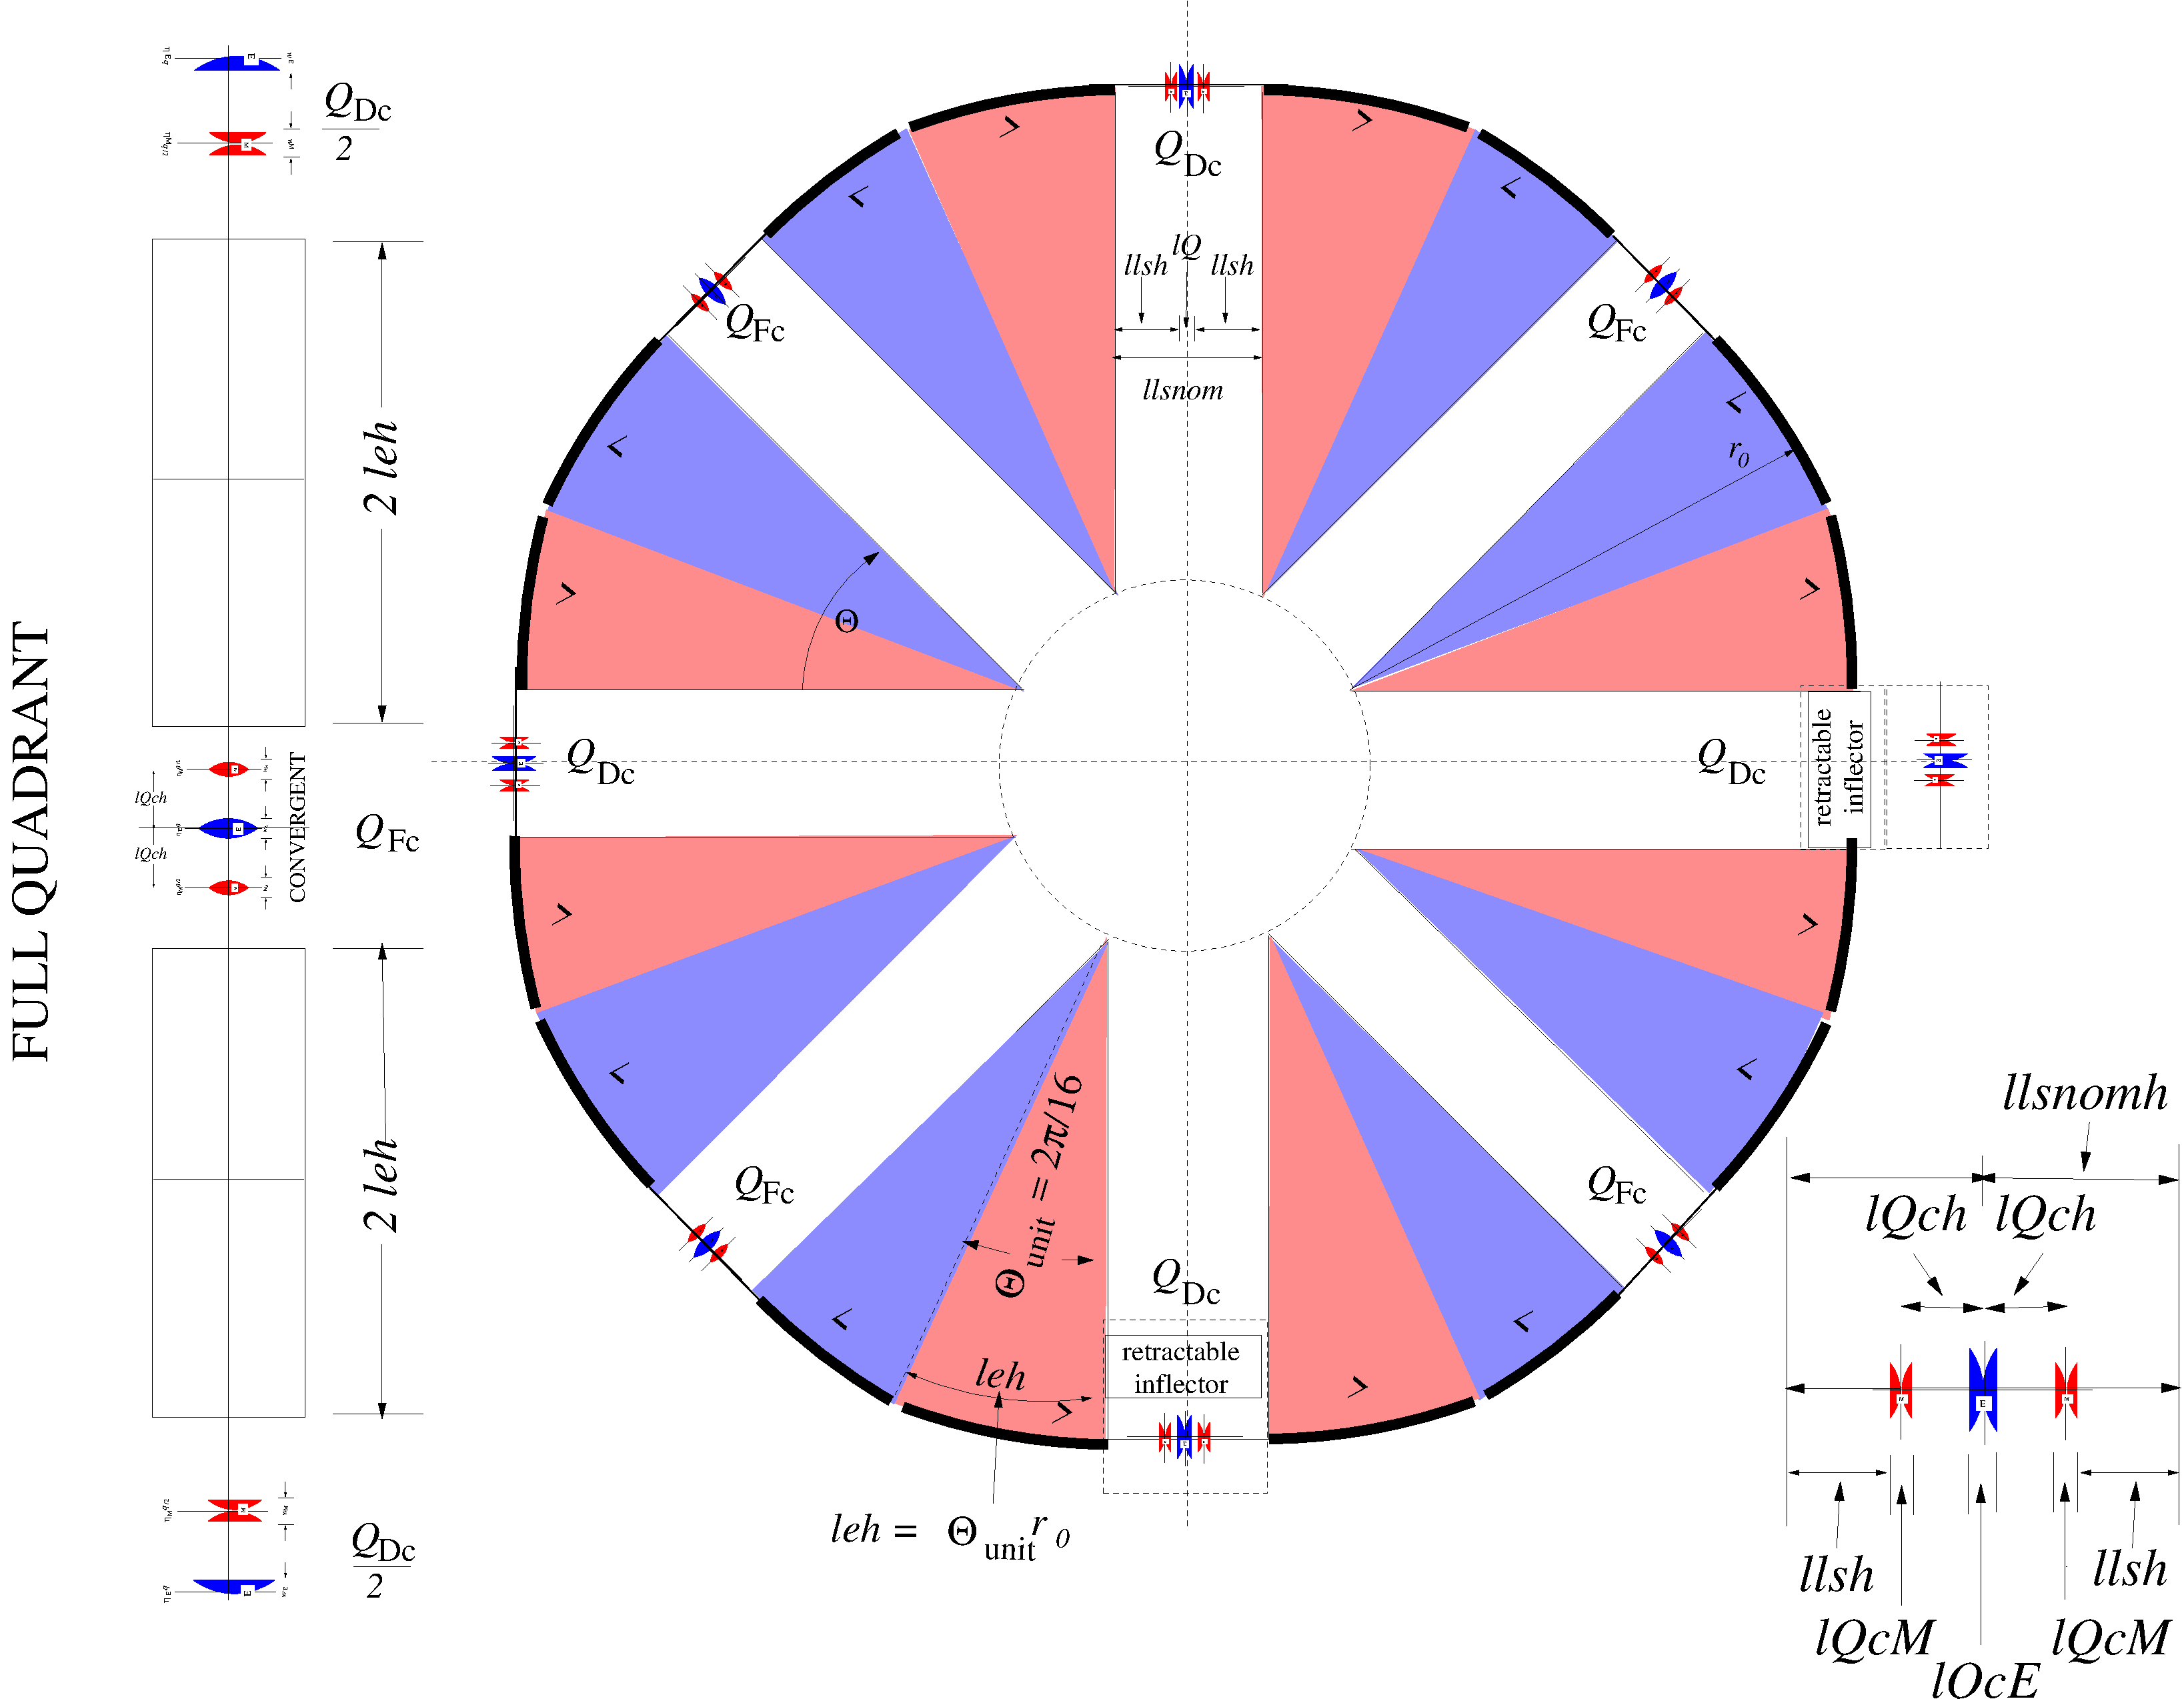
\includegraphics[scale=0.26]{pdf/PTR-layout-Toroidal8_102p2-mod.pdf}
\caption{\label{fig:PTR-layout-Toroidal8_102p2-mod}
Lattice layouts for PTR, the proposed prototype nuclear transmutation storage ring prototype;
The circumference has been taken to be 102\,m, but the entire lattice can be scaled, e.g. to 
reduce peak field requirements.  ``Compromise'' quadrupoles (shown lower on the right) are
located in each of eight long straight sections.  Detailed lattice files can be downloaded from GIT.
}
\end{figure}
%

For $m$=0 the fields are independent of vertical displacement $y$,
which implies that there is no vertical focusing provided by the bending field.
Provision of vertical stability therefore requires 
focusing quadrupoles; they are labeled $q$ in Figure~\ref{fig:PTR-layout-Toroidal8_102p2-mod}.
As well as being required for vertical stability, the $q$ quadrupoles are the only elents 
available in the control room for adjusting the optics of the storage ring.

%
\begin{figure}
\centering
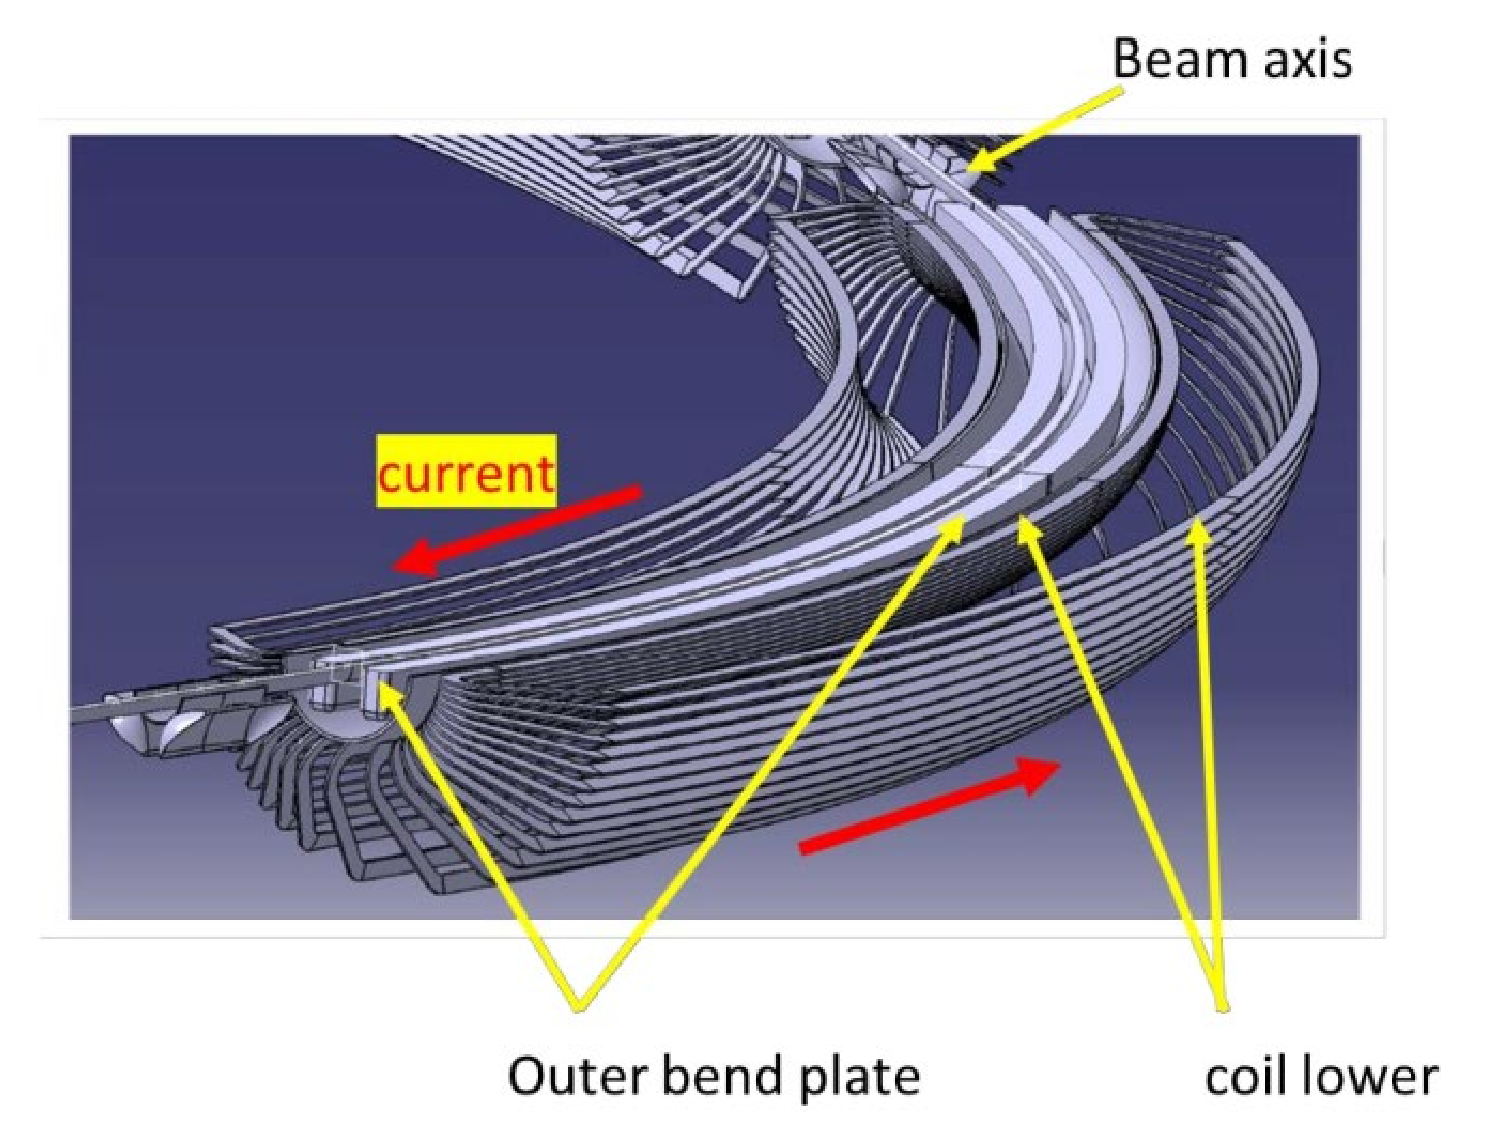
\includegraphics[scale=0.45]{pdf/Fig-5-bender.pdf}
\caption{\label{fig:SectorPerspective}Perspective mock-up of one sector of PTR, the superimposed 
E/M prototype ring. ``Short-circuited end'' cos\,$\theta$-dipoles surround the beam tube, within 
which are the toroidal capacitor plate electodes.  No magnetic field is superimposed in this benchmark.}
\end{figure}
%

\section{Parameters of Benchmark Lattices}
Lattice description files, with names like {\tt PTR\_m\_nom=0.32349-sl4.sxf}, 
readable by accelerator programs such as MAD or ETEAPOT, (and consistent with MAPLE 
parameterization of the same lattices) are located in the ``data'' 
directory.  These SXF lattice files are produced in {\tt /home/oxygen/XML2ADXF} and 
{\tt /home/oxygen/ADXF2SXF}.  Their (abbreviated) filenames are column headings in 
Table~{\ref{tbl:benchmarkParams.1}}, which contains lattice parameters and 
lattice properties such as tunes and beta functions determined by ETEAPOT.
For example, a related full lattice name is
``PTR\_m\_nom=0.29447-sl4.sxf''.  (The circumference is always contained in the final line of the lattice
``.sxf'' file.)  Later the ETEAPOT lattice prperties are to be compared with the same properties
calculated by MAPLE.  
%
\begin{table}[h]
\begin{tabular}{|c|c|c|c|c|c|c|c|c|}        \hline
                        & variable name         & unit & {\tt  PTR\_m=0.29447} & {\tt m=0.32349} & {\tt m=0.39447} \\ \hline
cells/arc         & {\tt NCellPerOctant} &        &       1                              &       1                    &        1                   \\
bend radius       &  {\tt r0}                 &  m   &     11.0                           &      11.0                &       11.0               \\
long drift length &  {\tt llsnom}         &  m   &         4.14214                  &     4.14214           &    4.14214            \\
half bend of cell & {\tt lh }                &  r    &         $2\pi$/16                  &      $2\pi$/16        &       $2\pi$/16        \\
half bend length  & {\tt leh}            &  m   &          $2\pi r0$/16             &    $2\pi r0$/16      &       $2\pi r0$/16     \\
circumference     & {\tt circum}      &  m   &      102.252179                &         102.252179  &   102.252179       \\ \hline
inverse focal length &  {\tt delq}     & 1/m  &     -0.009091                   &       -0.009091       &     -0.009091       \\
field index       &  {\tt m}                 &          &              0.29447             &       0.32349         &      0.39447          \\ \hline
horizontal beta  & {\tt betax}          &  m    &                                        &                             &                              \\
vertical beta     & {\tt betay}           &  m    &                                        &                            &                             \\ \hline
horizontal tune  &  {\tt Qx}              &        &                                         &                            &                              \\
vertical tune     &  {\tt Qy}               &        &                                         &                           &                                  \\
\hline
\end{tabular}
\caption{\label{tbl:benchmarkParams.1}Parameters of benchmark PTR lattices, 
and Twiss parameters (i.e. dynamic properties) calculated by ETEAPOT using linearized transfer matrices.  Note that 
ETEAPOT always ``slices'' each bend in the ``sxf'' file in half, before propagating sequentially through 
both slices.  This makes properties available at the bend center.} 
\end{table}
%

\section{Twiss Parameter Extraction}
A once-around (``monodromy'' in mathematical terminology) 
transfer matrix at any point in the ring has the standard Twiss parameterization,
%
\begin{equation}
{\bf{M}} =
  \begin{pmatrix}
           \cos\mu + \alpha \sin\mu &            \beta \sin\mu \\
   -\frac{1+\alpha^2}{\beta}\sin\mu & \cos\mu - \alpha \sin\mu
  \end{pmatrix}.
\label{eq:Twiss.1}
\end{equation}
%
At a mirror symmetry point in the lattice, as at present, though not in general, $\alpha$ vanishes.
The phase advance $\mu$ = 2$\pi Q$ can be obtained from
%
\begin{equation}
 \cos\mu=\frac{M_{11}+M_{22}}{2}, \quad \hbox{and} \quad M_{12}=\beta \sin\mu.
\label{eq:Twiss.2}
\end{equation}
%
This has assumed that $\beta$ is, by definition, positive.
These equations determine the signs of both $\cos\mu$ and $\sin\mu$. Reading counter-clockwise, the four 
consecutive phase space quadrants, I/II/III/IV, are characterized by cosine, sine sign pairs 
++/-+/- -/+-, respectively. We then obtain the fractional parts of the phase advance from 
%
\begin{equation}
 \mu = 
\begin{cases} 
       \cos^{-1}( \frac{M_{11}+M_{22}}{2} ), & \mbox{if } \textnormal{quadrant}\mbox{ is I or II} \\ 
  2\pi-\cos^{-1}( \frac{M_{11}+M_{22}}{2} ), & \mbox{if } \textnormal{quadrant}\mbox{ is III or IV} \end{cases}.
\label{eq:Twiss.3}
\end{equation}
%
This still only partially resolves the aliasing ambiguity. Resolving the integer tune ambiguity requires 
keeping track of phase space quadrants while tracking through the lattice. To avoid error in this
process it is important for sampling intervals small enough that no phase quadrant can be skipped.
This keeping track of the integer tune is indicated in captions 
to graphs below. We then obtain $\beta$ from Eq.~(\ref{eq:Twiss.2}), and $\alpha$ from 
%
\begin{equation}
 \alpha=\frac{M_{11}-M_{22}}{2\sin\mu}.
\label{eq:Twiss.4}
\end{equation}
%
It is because the TEAPOT family of codes use only particle tracking, and no transfer matrices in
studying ring behavior---transfer matrix components, and Twiss and other lattice functions are only 
obtained for the purpose of comparing results with more conventional accelerator simulation codes.

\section{ETEAPOT tune determinations and analytic comparisons}
\subsection{Data collection organization}
In all cases, $m=0.29447, 0.32349, 0.39447$, the lumped Q-quadrupoles strengths, $delq$, were adjusted
to a ``nearly-off'' state, just strong enough to produce vertical stability in all cases.
For each of the three benchmark lattices, bunches of 21 standard particles are 
tracked for ten turns. Each of the bend elements is sliced in half for this (and all other) analyses. 
The graphs show horizontal and vertical displacements for two of the standard particles at the exits from 
each turn.  Both transverse tune determinations are shown in the figure captions. 

The reason for tracking a significantly large number of turns (10), is to avoid ``aliasing'' problems which will
be explained later.

Once-around transfer matrices are obtained from the 21 standard particles using numerical differences. 
This differencing is based on the smallness (typically 1\,$\mu$m spatial displacement, 1\,$\mu$r 
angular displacement) of the initial offsets.  Sensitivity to this choice has been investigated previously.
Twiss parameters, $\beta_x, \beta_y$, and  $\mu_x, \mu_y$ are calculated using the procedures already 
described. The fractional and integer tune values are obtained from the graphs.

Each bend element in any SXF lattice description file corresponds to a single bend element in
an actual ring and is therefore referred to as a ``single bend''. By the internal construction of ETEAPOT, 
each such bend is sliced at least once, and (optionally) more times. 

\subsection{PTR lattice tracking tune determinations}
The following figures exhibit the determination of horizontal and vertical tunes $Q_x$ and $Q_y$  for each of 
the three lattices under study, by counting the number of betatron oscillations occuring after ten
complete revolutions.  The arithmetic is completed in the figure captions.
%
\begin{figure}[htbp]
  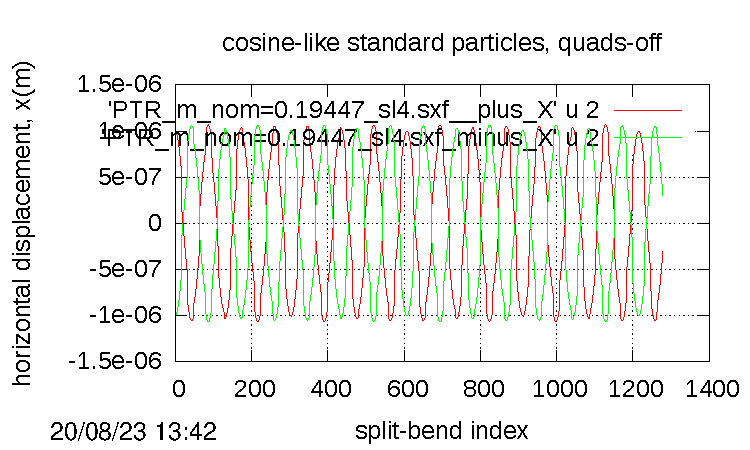
\includegraphics[scale=0.65]{pdf/Fig-p19-t.pdf}
  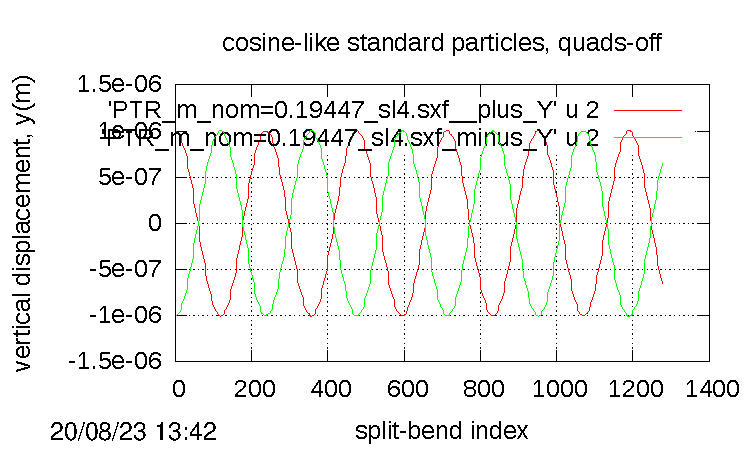
\includegraphics[scale=0.65]{pdf/Fig-p19-b.pdf} 
\caption{Lattice {\tt PTR\_m\_nom=0.19447-sl4.sxf}; Upper: horizontal Displacement: 10 turns, 
1 sample per split bend; $Q_x\approx$ 15.2 osc/10turns=1.52 osc/turn; the horizontal tune is $Q_x$= 1.52. 
Lower: vertical Displacement: 10 turns. $Q_y\approx$ 
5.4 osc/10turns=0.54 osc/turn. The vertical tune is $Q_y$= 0.54.}
\end{figure}
%
%
\begin{figure}[htbp]
  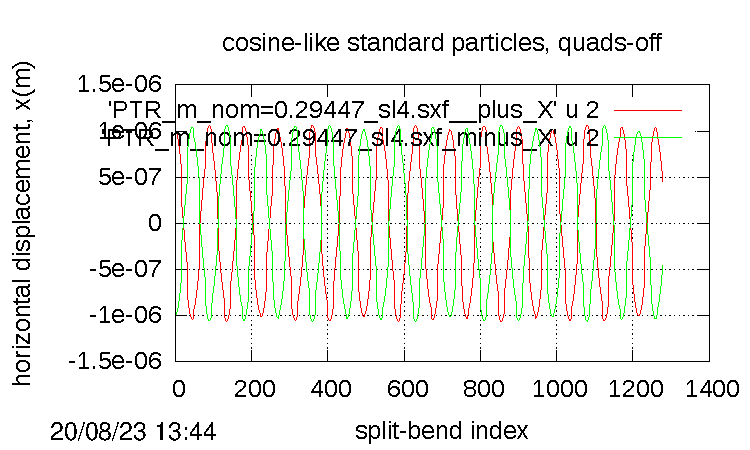
\includegraphics[scale=0.65]{pdf/Fig-p29-t.pdf}
  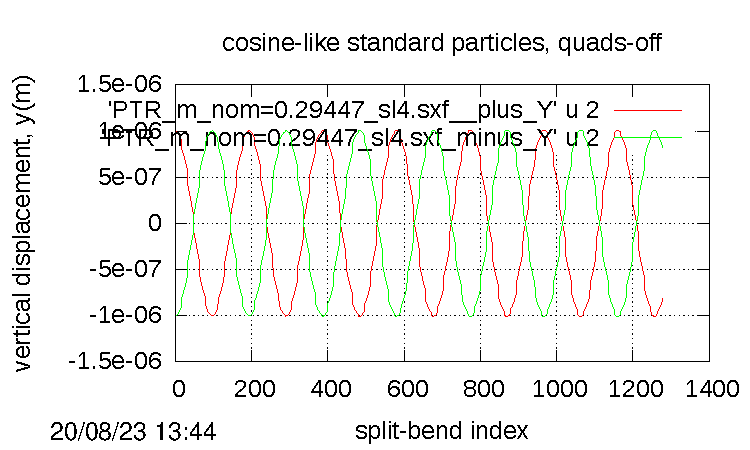
\includegraphics[scale=0.65]{pdf/Fig-p29-b.pdf} 
\caption{Lattice {\tt PTR\_m\_nom=0.29447-sl4.sxf}; Upper: horizontal Displacement: 10 turns, 
1 sample per split bend; $Q_x\approx$ 14.2 osc/10turns=1.42 osc/turn; the horizontal tune is $Q_x$ = 1.42. 
Lower: vertical Displacement: 10 turns. $Q_y\approx$6.55 osc/10turns=0.655 osc/turn. The vertical tune is $Q_y$ = 0.655.}
\end{figure}
%
%
\begin{figure}[htbp]
  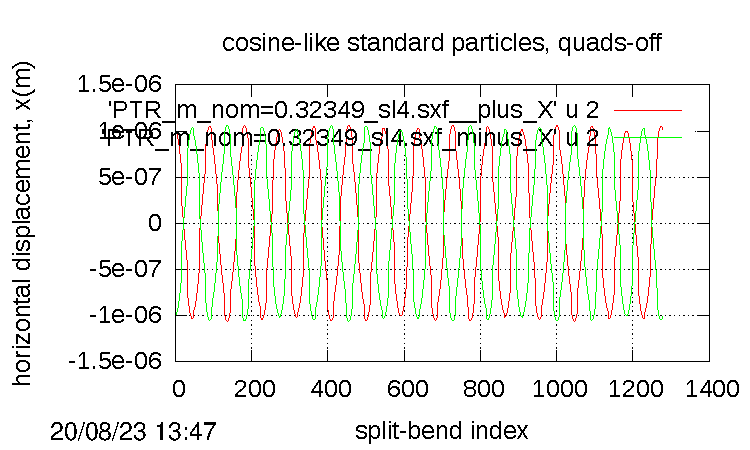
\includegraphics[scale=0.65]{pdf/Fig-p32-t.pdf}
  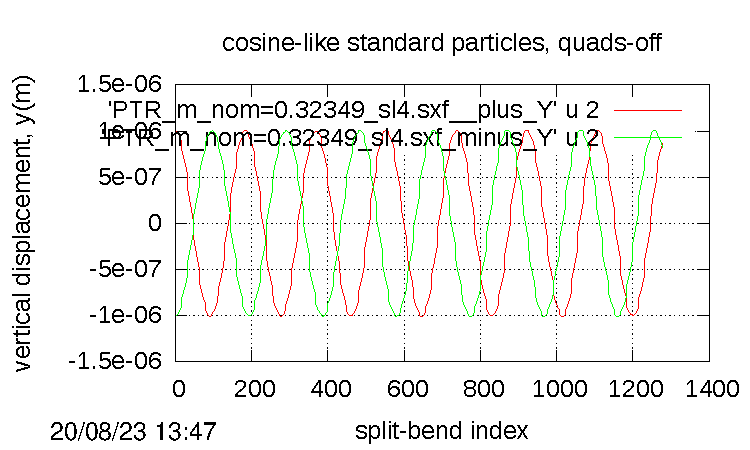
\includegraphics[scale=0.65]{pdf/Fig-p32-b.pdf} 
\caption{Lattice {\tt PTR\_m\_nom=0.32349-sl4.sxf}; Upper: horizontal Displacement: 10 turns, 
1 sample per split bend; $Q_x\approx$ 14.0 osc/10turns=1.40 osc/turn; the horizontal tune is $Q_x$ = 1.40. 
Lower: vertical Displacement: 10 turns, 1 sample per split bend. $Q_y\approx$6.55 osc/10turns=0.655 osc/turn. 
The vertical tune is $Q_y$ = 0.655.}
\end{figure}
%
%
\begin{figure}[htbp]
  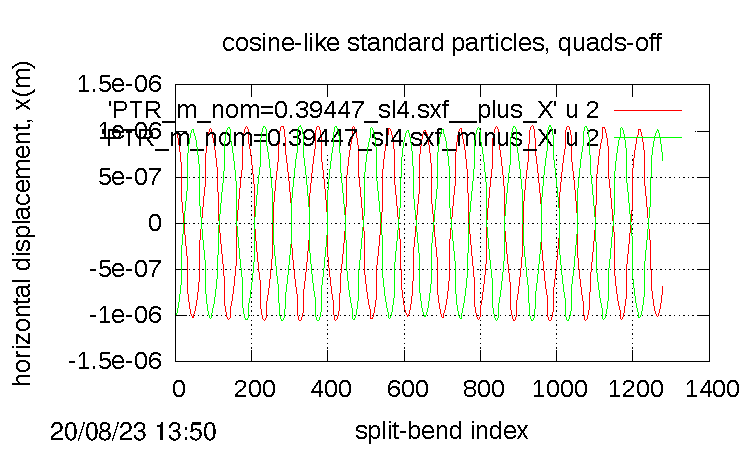
\includegraphics[scale=0.6]{pdf/Fig-p39-t.pdf}
  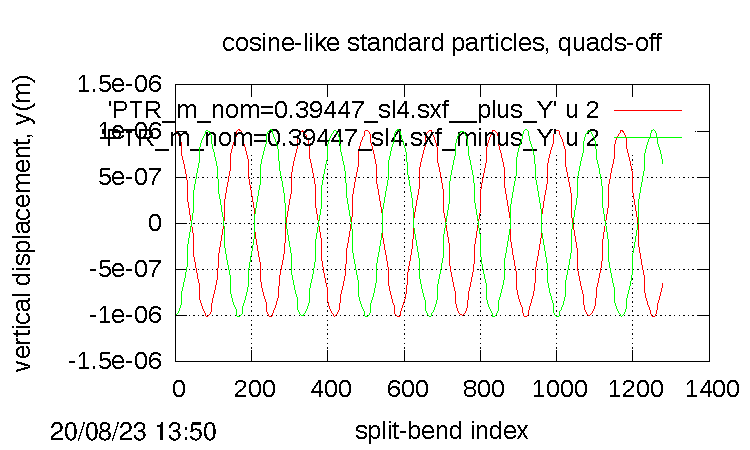
\includegraphics[scale=0.6]{pdf/Fig-p39-b.pdf} 
\caption{Lattice {\tt PTR\_m\_nom=0.39447-sl4.sxf}; Upper: horizontal Displacement: 10 turns, 
1 sample per split bend; $Q_x\approx$ 13.55 osc/10turns=1.355 osc/turn; the horizontal tune is $Q_x$ = 1.355. 
Lower: vertical Displacement: 10 turns, 1 sample per split bend. $Q_y\approx$ 
7.6 osc/10turns=0.76 osc/turn. The vertical tune is $Q_y$ = 0.76.}
\end{figure}
%
%
Table~\ref{tbl:benchmarkParams.P1.0} shows the lattice parameters obtained
with $m=1$, ``spherical'' bending, with minimal ETEAPOT slicing of 2 slices per bend.
ETEAPOT results agree well with analytic lattice calculations using MAPLE. The 
accuracy of ``differentiation by differencing'' is investigated. The effect of
increasing the unit differencing value ${\tt tiny}=10^{-6}$ by two orders of manitude
has negligible effect on the lattice parameters, showing that the differencing provides
sufficient accuracy.

\begin{table}[h]
\begin{tabular}{|c|c|c|cc|cc|cc|}           \hline
program                    &                        &       &    MAPLE  &  ETEAPOT &   MAPLE  &  ETEAPOT  &  MAPLE    &  ETEAPOT     \\ \hline
field index                 &    $m$             &       &  0.29447 &   0.29447  & 0.32349  &  0.32349    &  0.39447 &  0.39447       \\ \hline 
horizontal beta         & {\tt betax}      &  m &                 &                  &                &                   &                &                      \\
vertical beta             & {\tt betay}      &  m &                 &                  &                &                   &                &                      \\  \hline 
horizontal tune         &  {\tt Qx}         &       &                 &     1.42      &                &    1.40        &                &    1.355         \\ 
vertical tune             &  {\tt Qy}         &       &                 &     0.655    &                &    0.655      &                &    0.76           \\  \hline
\end{tabular}
\caption{\label{tbl:benchmarkParams.P1.0}Comparison of ETEAPOT and MAPLE tune results.  Spaces left blank are to be filled in
in subsequent benchmark tests, which will also produce more acccurate values.   All numerical differentiation displacements 
in ETEAPOT are takn to be {\tt tiny}=$10^{-6}$\,m.}.  The calculational parameter ``{\tt tiny}'' can be increased by at least 
two orders of magnitude without changing the results significantly.
\end{table}
%

\section{Comments and Conclusions}
ETEAPOT tracking was initially based on an analytical relativistic astronomical Kepler planetary orbit formulation of 
Munoz and Pavic, listed along with other relevant formulations in the bibliography below.  Since this analytic approach was
quite unwieldy it was eventually replaced more in the pirit of the original TEAPOT code.  The introduction of superimpoed 
magnetic bending rules out any cloed form analytic approach.

We refer to ETEAPOT orbit tracking as representing  a ``Schr\"odinger Picture'' determination of beam evolution in a 
storage ring.  Calculated using classical (relativistic) mechanics, in a wave-like picture of particle evoluting with $s$, 
these ``eikonal curves'', calculated as in geometric optics, are orthogonal to wavefronts in a Schr\"odinger wave 
propogation picture.  These rays can be used to calculate lattice beta functions as ``ray envelopes'' in following 
benchmark investigations. 

The (MAPLE) BSM code treats the beam transfer matrices, whose elements are expressed in terms of beta functions.
as evolving with $s$ in a ``Heisenberg-like'' picture  
 

FOLLOWING is NOT YET UPDATED to PTR lattice

For the $m=1$ case, there is nearly exact agreement between the linearized analytic formulae and the tracking formalism. 
This is ``as should be'', but far from automatic. The equations of the linearized transfer matrix formalism and the 
arbitrary-amplitude Munoz-Pavic seem utterly different. So the close agreement confirms \emph{both} approaches.
This comment mainly applies to the ``in-plane'' horizontal motion. Agreement of the ``out-of-plane'' vertical
motion, where the overall agreement is less impressive, especially as investigated with a pre-sliced SXF lattice,
in Sections~\ref{sect:pre-sliced} and \ref{sect:pre-sliced-modQ}. Vertical steering errors, however small, are 
amplified by the weak vertical focusing of the lattice. 

The agreement for $m\ne1$ is excellent, but clearly not as good as for $m=1$. This strongly suggests that the 
(artificial) perturbative kick compensation is not quite perfect. It is also not surprising that the deviation 
is proportional to $(m-1)^2$; and that, for $m=1$, the kick correction strength vanishes.

For most practical purposes, the code performance in the parameter range $-1\le m\le 1$ has been shown to 
be satisfactory. 

\clearpage

\begin{thebibliography}{99}
\bibitem{pEDM}
Storage Ring EDM Collaboration, \emph{A Proposal to Measure the
Proton Electric Dipole Moment with $10^{-29}\,$e-cm Sensitivity,}
especially Appendix 1. October, 2011

\bibitem{Moller}
C. M\o ller, \emph{The Theory of Relativity,} Clarendon Press,
Oxford, 1952, 

\bibitem{Munoz}
G. Mu\~{n}oz and I. Pavic, \emph{A Hamilton-like vector for
the special-relativistic Coulomb problem,} 
Eur. J. Phys. {\bf 27}, 1007-1018, 2006

\bibitem{Talman}
R. Talman, \emph{Geometric Mechanics,} John Wiley and Sons, 2000

\bibitem{Aguirregabiria}
J. Aguirregabiria et al., 
Archiv:physics/0407049v1 [physics.ed-ph] 2004, 

\bibitem{Torkelsson}
U. Torkelsson, Eur. J. Phys., {\bf 19}, 459, 1998, 

\bibitem{Boyer}
T. Boyer, Am. J. Phys. {\bf 72} (8) 992, 2004

\end{thebibliography}


\end{document}

